\chapter{System Validation}
This chapter will go into detail about the testing and evaluation performed during and at the conclusion of the development process. Various forms of testing were performed during the development of each component in the iterative sprints set out with the scrum methodology.

\section{Testing}
	\subsection{Unit Testing}
	Unit testing was only used for one component of the system; the storage server. The storage server was the most suited towards this  testing approach as it is composed of deterministic API methods. The unit testing was performed using Flask's built-in unit testing functionality that is based on the built-in unittest Python package.

	Unit tests were created to perform each API route in a stable environment; this was achieved by first creating a new repository through the API, performing the related test for each functionality, then deleting the repository. A total of 8 unit tests were created, one for each API route on the storage server. The results for each unit test was a pass at the end of the development iteration for the storage server.

	\subsection{Test Game}
	A test game was created to test the development of the game engine. The test game was constructed manually in the gamedata JSON structure, specifying several entities with components, each of which would test a specific component and their interactions. This was used during each game engine sprint to make sure any changes implemented were functioning correctly.

	\subsection{White Box Testing}
	White box testing was performed on each component in the system, by constructing HTTP requests that would attempt to cause an error on the system. This was done using the \textbf{curl} command, as some requests would require sending extra data or using a request method such as POST or DELETE. This was done for each new route created on the web and storage servers, and assisted greatly in making them as stable as possible.

	\subsection{Integration Testing}
	Integration testing was performed when integrating two systems together. This was performed when constructing the communications class between the web server and storage server, as well as implementing the game engine into the game editor. A top-down testing approach was used while doing the integration testing, testing the highest level of the systems and moving down towards the low level operations as the testing proceeded.

	\subsection{Regression Testing}
	After each sprint iteration, the changes that were implemented such as features or fixes, were tested heavily to find any new bugs that may have been introduced along with them. This was completed using functional testing by feeding valid data into each component and seeing if any unwanted behaviour occurred. The unit tests created for the storage server were also utilised during this process.

\section{Evaluation}
	\subsection{Usability}
	The usability of the developed system was evaluated using the IxD checklist, a tool that is used to quickly evaluate websites for usability issues. The system was evaluated using all categories of the IxD checklist, including the interface, typography, iconography, interaction and navigation categories. Each category selected adds several check boxes to the checklist, in different usability areas.

	The checklist was completed by evaluating the system vs each checklist item, with the items being usability guidelines such as `The controls map to the result in a simple and logical way' and `Current state of the system is easily understood by the user'. If the guideline is passed, then the checkbox for that item is ticked.

	% todo ref ixd & quotes

	Out of the 28 items on the list, 7 items were not ticked. The sections with the most unpassed items were in the simplicity, tolerance and accessibility areas of the checklist. This indicates that the while the user may understand the interfaces, and can use the system, it's not as easy as it could be. Adding a page providing `help and support', and controls for undoing actions would help improve the usability of the system greatly.

	\subsection{Performance}
	The performance and memory usage of the game editor and game engine were evaluated and compared to existing platforms as a baseline.

	\paragraph{Memory usage}
	The memory usage of the editor was rather significant, hitting about 140 megabytes of memory on average, compared to the homepage of the website which only uses 20 megabytes. However, the memory usage of a commercial website such as Facebook, which averages around 200 megabytes of memory, shows that the editor is still quite efficient at memory management. The memory usage of a sample game uses only around 115 megabytes of memory.

	\paragraph{Page loading speed}
	The loading speed of several pages were tested, with the slowest page being the editor; as it can loads over 34 files. It takes about 800 milliseconds for the editor content to load fully (without caching). Using the PageSpeed test on the Google Developers website, the website was tested to determine if this could be improved. The result of the PageSpeed test (Figure \ref{fig:pagespeed}) showed that the page size could be reduced significantly (by 78\%) by adding `compression' to the server. A Flask plugin called Flask-Compress was found that can implement this rather easily. Adding it to the web application improved the loading speed of the editor down to only 500 milliseconds total, compared to Facebook which can take up to 5 seconds to load fully.

	% todo ref:
	% https://developers.google.com/speed/pagespeed/insights
	% https://flask-compress.readthedocs.org/en/latest/

\begin{figure}[h]
	\centering
	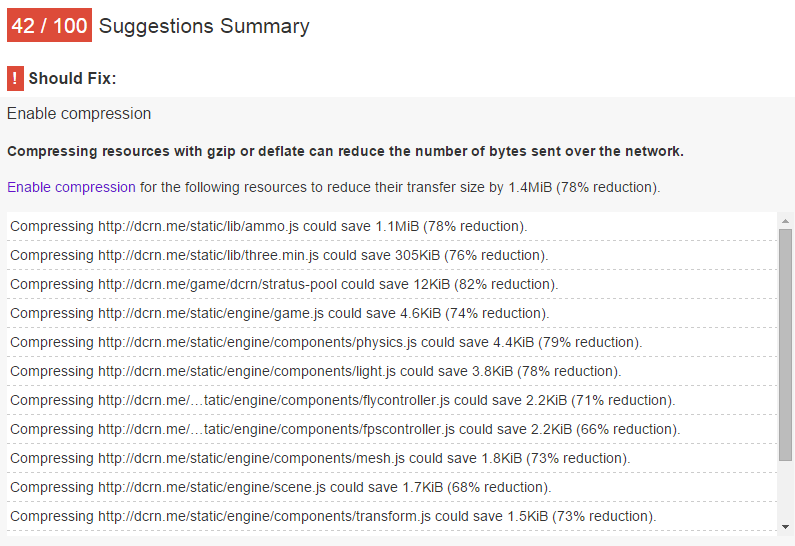
\includegraphics[scale=0.5]{compression}
	\caption{Google Developers PageSpeed test result}
	\label{fig:pagespeed}
\end{figure}

	\paragraph{Frames per second}
	The framerate of the game engine was evaluated using Google Chrome's built-in `FPS Counter' which is disabled by default. The FPS counter can be enabled to show the current amount of frames per second on the page, which provides a good measure of how well a game is performing. A framerate of 60 frames per second is the standard for the majority of video games, with most computer monitors only supporting up to 60hz.

	Several games were tested on two computers (Windows and Linux), with the majority of the games giving a solid 60 frames per second on both machines. Instances of lower frames per second (\~40) were observed when the number of physics entities was very high, but only when all of them were active and moving around the scene. This shows that having a large amount of moving physics objects will reduce the performance of the games significantly, but this can be resolved by using as many static physics objects as possible. Shadows can also cause a performance loss, but these can be tweaked to have a different `type' (Soft, basic) in the game settings, which can improve the performance of shadows at the cost of quality.

	\subsection{Compatibility}
	The compatibility of the game engine was tested using multiple devices and internet browsers. The result of this was that the game engine performs perfectly on the Google Chrome browser, while running with a slightly lower performance on the Mozilla Firefox browser.

	The game engine's performance on an android tablet device was also checked, in the hopes it would even run at all. The result was surprising in that it worked perfectly, but the performance was quite very low, running at around 15 frames per second on the Nexus 7 2012 tablet. It may be possible to create games targeted to Android devices by using very few physics objects and no shadows.

	\subsection{User Testing}
	User testing was performed with a group of 7 people, each with experience in different domains such as Engineering, Computer Science and Game Design, which gave a good variance of experience coming into the testing. Users were instructed to attempt to make a game and publish it, and were given no instructions on how to do this, letting them figure it out for themselves.

	A survey was created to collect and aggregate the results of each user's experience with the system. The user was asked to fill in the details of their experience, including the usability of the interface, the ease of creating games and publishing them, using JavaScript to create components, and how the system compared to other applications such as Unity and Unreal Engine.

	The results of the survey (Available in Appendix \ref{appendix:survey}) showed that the users had an overall good experience on the system. The usability of the interfaces was generally easy to understand and provided feedback where possible. The editor was easy to use for the creation of games, but users had difficulty in creating new components using JavaScript; especially those who had no experience using JavaScript before. This is most likely due to the lack of a complete API and documentation for creating new components.

	Compared to other game engines, some users found Stratus to be lacking, this was most common with users who had previously used other game engines such as Unity and Unreal, but didn't have very much experience in using them. This is understandable, as Stratus lacks some major features that are important to game design, including materials, custom models and terrain geometry.

	The users were also asked to provide some feedback and suggested features, or any issues they ran into during their experience with Stratus. The first user to complete the user testing gave some simple but very important feedback; that was to add a default camera to every new scene. It was agreed that this would make it easier for users with less experience, and it was implemented into the editor immediately. For the rest of the user testing, this was available and assisted them in creating games.

	After that, the most common feedback was that it was difficult to set specific values on on the sliders for position, scale and rotation. Adding in an input box with the specific value beside each slider would assist with this, allowing users to input the value they want. This is a feature that would be very useful in the editor interface, and is planned for future developments.

\section{Demonstration}
% Identify what features can be demonstrated and show screenshots or reference a video online to show the project demonstration
% TODO!